\chapter{Objectifs et démarches}\label{chap:mod}
%Dans le cadre de l'élaboration de notre modèle, trois méta-modèles ont été mis à notre disposition par \kwobeo. Dans ce chapitre, nous détaillerons le rôle de ces trois méta-modèles.


\section{Objectifs}
Dans le cadre du module \emph{SC Project}, nous avons eu l'opportunité de travailler sur la conception d'outils de modélisation dédiés aux applications web. En partant de trois méta modèles mis à disposition par \textsc{Obeo}
(\cf{} section \ref{chap:tra}) l'objectif était de créer des modèles et les générateurs de code pour produire le code d'une application. L'utilisateur final aura ainsi la possibilité de créer le modèle de son application web (à partir d'une vue en arbre par exemple) puis d'exécuter le générateur mis à disposition pour produire le code de l'application désirée.



\section{Démarche} 

Les premières semaines du projet furent consacrées à la prise en main des outils et des technologies. S.\textsc{Thibaudeau} nous a mis à disposition des exemples de générateurs et les références vers les différentes initiations indispensables pour ce projet (Tutoriel Acceleo, ObeoDesigner~\dots). En parallèle nous avons aussi étudié le framework \kwplay{} et vérifié la compatibilité avec l'objectif de ce projet.

\begin{figure}[htb]
  % \centering
  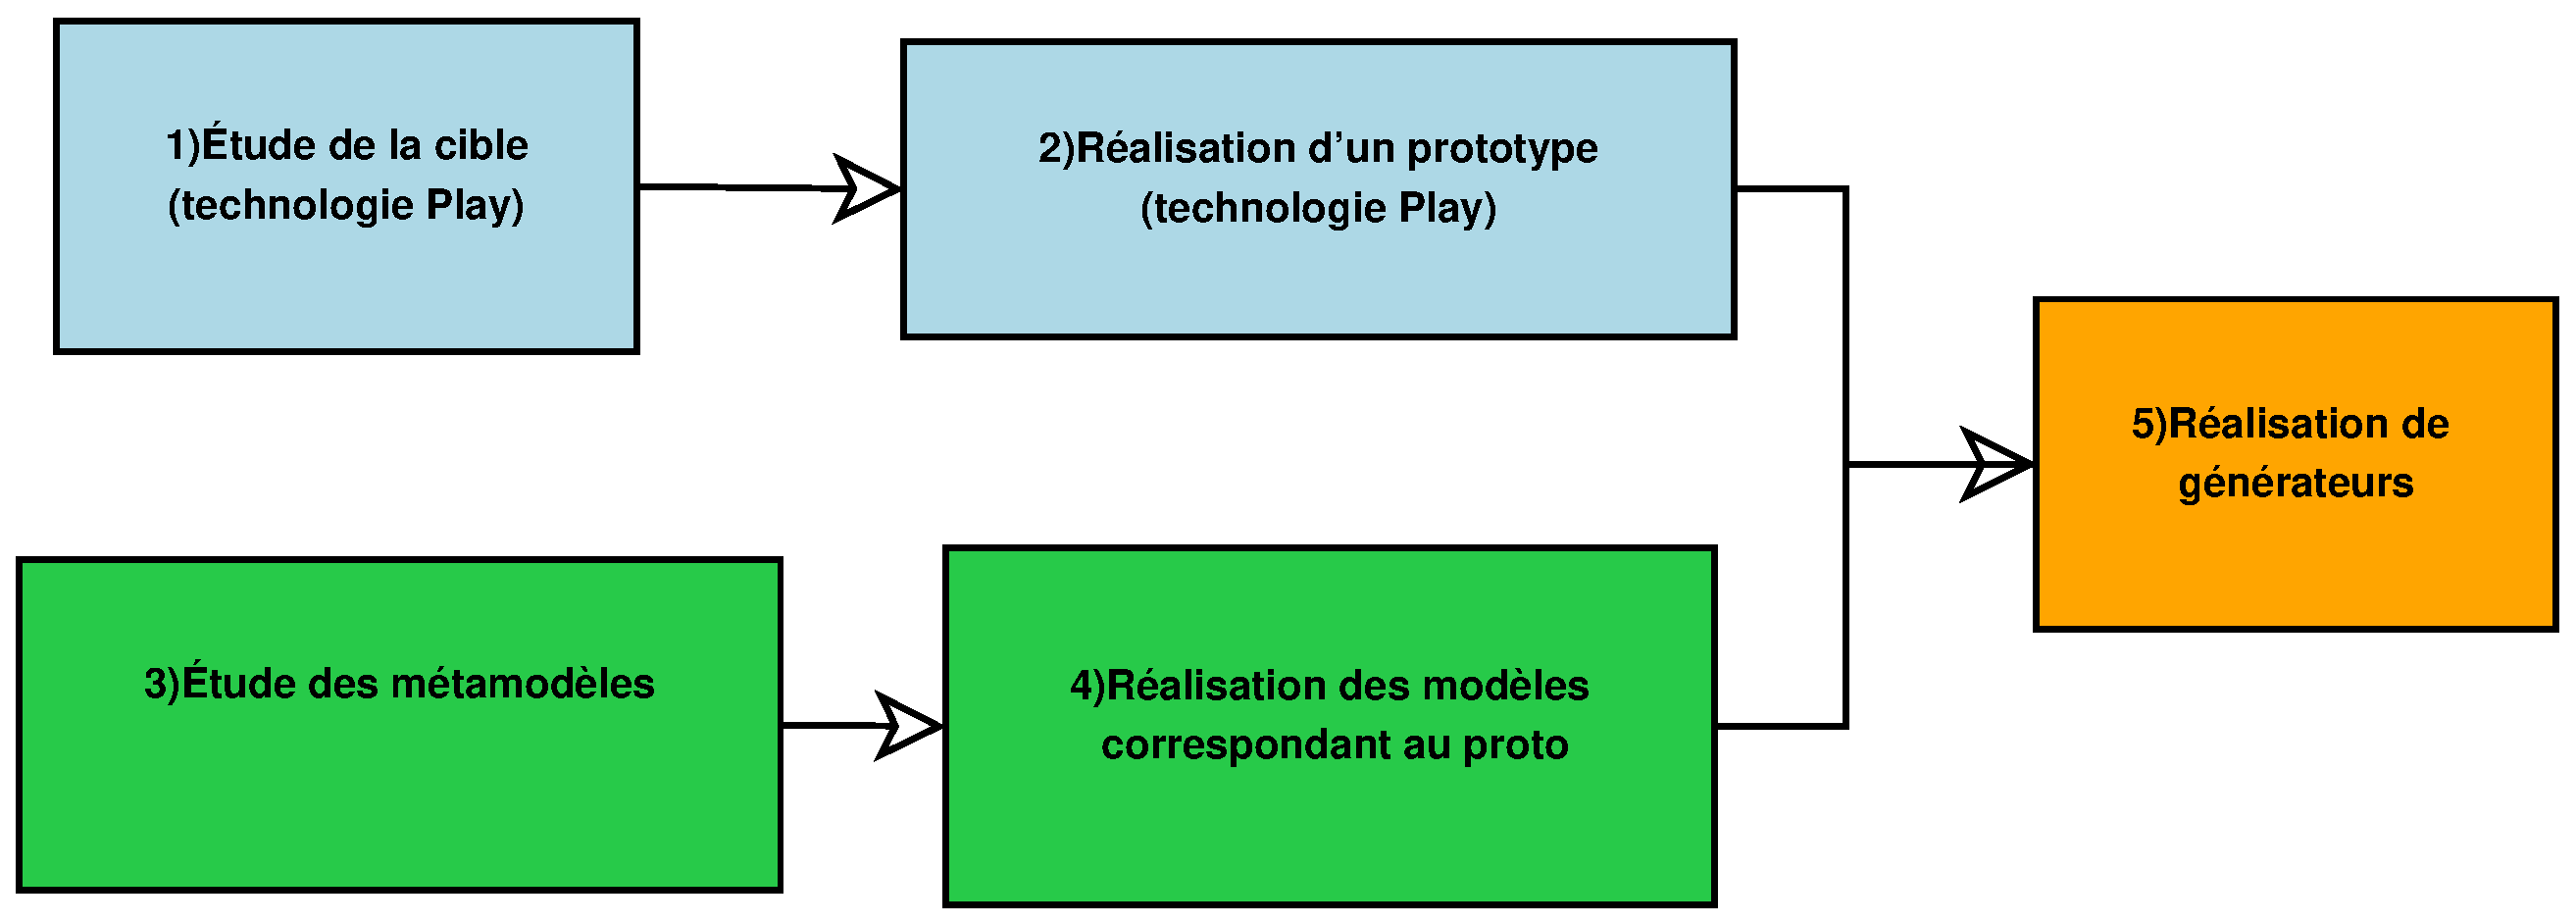
\includegraphics[scale=.4]{img/demarche.eps}
  \caption{Démarche employée}
  \label{fig:dem}
\end{figure}

Dans un second temps, nous avons entamé la conception d'un prototype d'une application web avec \kwplay{}. Enfin, nous avons étudié les différents méta-modèles mis à disposition puis entamé la création des différents générateurs de code associés. Dans ce rapport nous détaillerons ces différents étapes du projet. Ainsi le chapitre \ref{chap:met} résume l'étude menée sur le \kwplay{} et le prototype créé. Dans le chapitre \ref{chap:tra} nous reviendrons sur les différents méta-modèles ainsi que les générateurs de code associés. 

\paragraph{Outil de gestion de version}


Comme la plupart des projets à l'initiative de l'entreprise \kwobeo, ce projet est \textit{Open Source}. Afin de partager et collaborer, S.\textsc{Thibaudeau} nous a proposé d'utiliser \emph{Github} (\cf{} \cite{git}).%
\begin{figure}[htb]
  \centering
  
\includegraphics[scale=.3]{img/git.eps}
\end{figure}
Nous avons créer un compte \href{alma2012}{https://github.com/alma2012} dédié à ce projet.


% LocalWords:  méta-modèles SC Project web Obeo Thibaudeau Tutoriel
% LocalWords:  Acceleo ObeoDesigner framework
